% Chapter Template

\chapter{Introduction and Motivation} % Main chapter title

\label{Chapter1} % Change X to a consecutive number; for referencing this chapter elsewhere, use \ref{ChapterX}

%----------------------------------------------------------------------------------------
%	SECTION
%----------------------------------------------------------------------------------------

\section{Introduction}

In many modern-day applications and computer programs, we may encounter frequently a situation where users have to browse or interact with a large set of data or information, however, only focusing only on a certian part of them. In many situations, this part is usually a lot smaller than the original dataset relatively. The most commonly seen scenario would be a \gls{gis} programs on computers, for example an \gls{opd} display shown in \gmref{fig:usgsmap}. These type of applications usually have a zoomable interface to allow users to zoom into a specific region of the original dataset. Also they usually allow users to browse around the dataset from the current focus region and navigate and interact with the whole large dataset with the sense of the ``large picture'' by the mechanism of \gls{opd} techniques.

\begin{figure}[th]
\centering
% 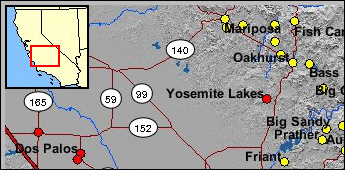
\includegraphics[width=\textwidth,keepaspectratio]{Figures/Chapter1/usgsmap.png}
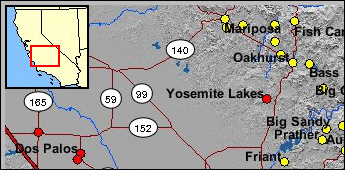
\includegraphics{Figures/Chapter1/usgsmap.png}
\decoRule
\caption[Overview Plus Details On Map]{From \url{http://wildfire.usgs.gov}, an overview of the graphics next to a zoomed ``detail view''.}
\label{fig:usgsmap}
\end{figure}

Other examples besides \gls{gis} include also some image processing, image generation applications such as Photoshop shown in \gmref{fig:ps}, because usually the resolution of the image being processed or generated are larger than the resolution of one single screen monitor. Another interesting example would be in the modern computer gaming industry, that the concept of \emph{Mini-map}s were invented, illustrated in \gmref{fig:minimap}, with the same concepts due to the fact that the virtual world of digital games are mostly a lot larger than how much one single screen can contain.

\begin{figure}[th]
\centering
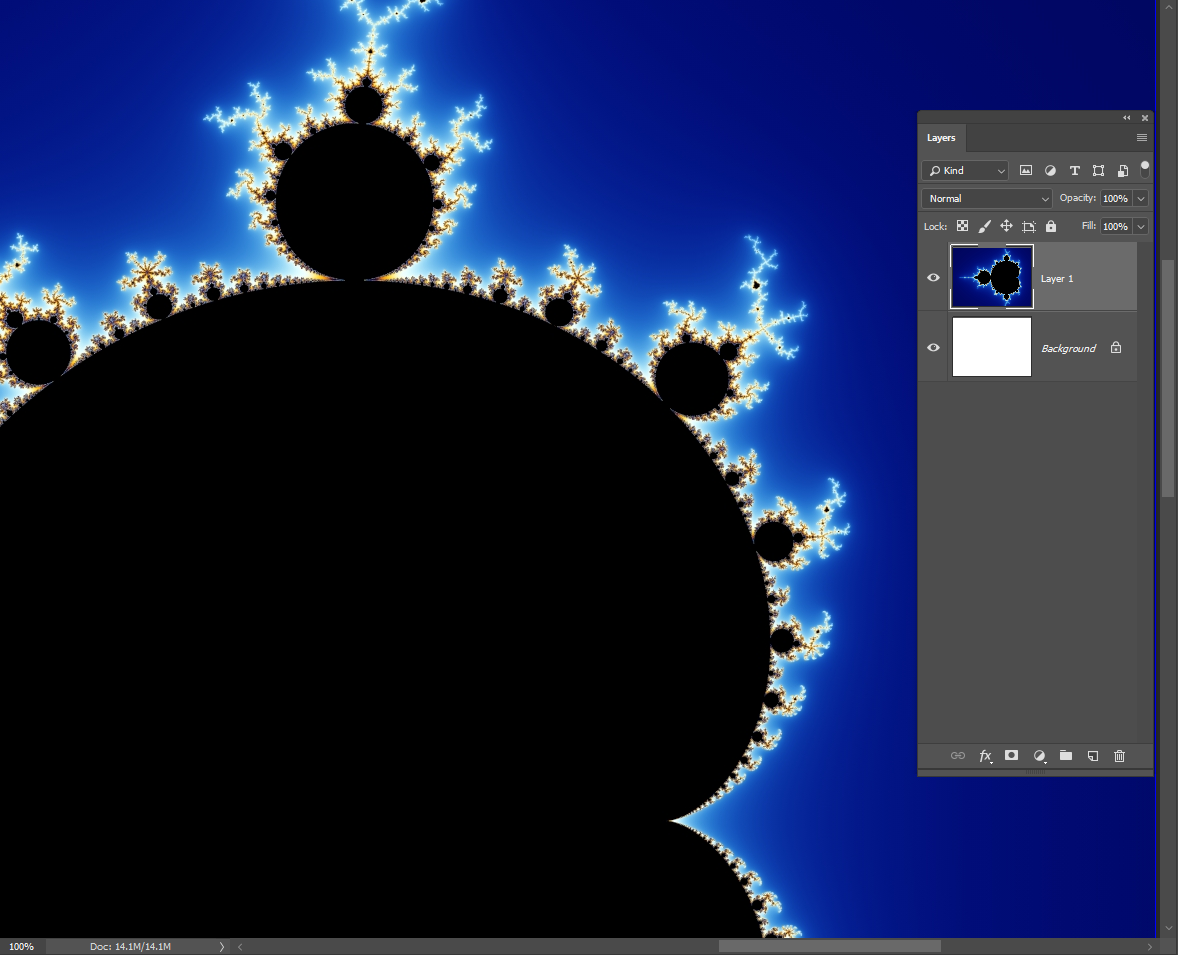
\includegraphics[width=\textwidth,keepaspectratio]{Figures/Chapter1/ps.png}
% 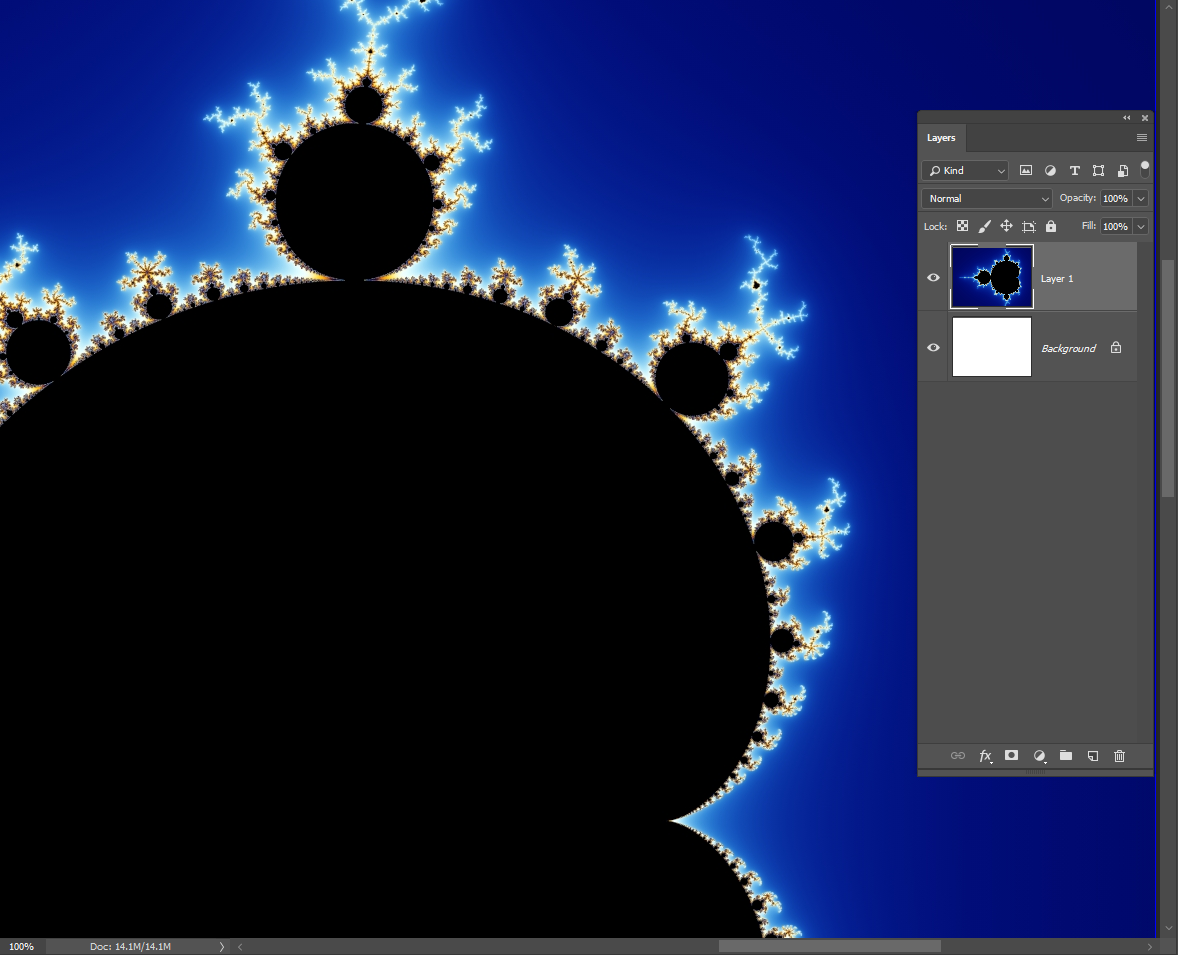
\includegraphics{Figures/Chapter1/ps.png}
\decoRule
\caption[Overview Plus Details In Photoshop]{The basic mechanism in the application Photoshop, layers, offering an overview functionality, with detailed focus area on the main visual area.}
\label{fig:ps}
\end{figure}

\begin{figure}[th]
\centering
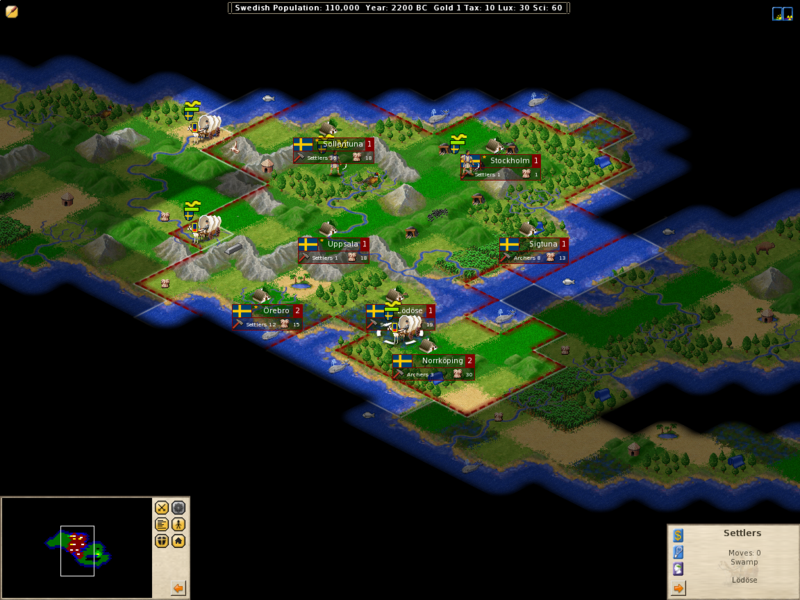
\includegraphics[width=0.65\textwidth,keepaspectratio]{Figures/Chapter1/minimap.png}
% 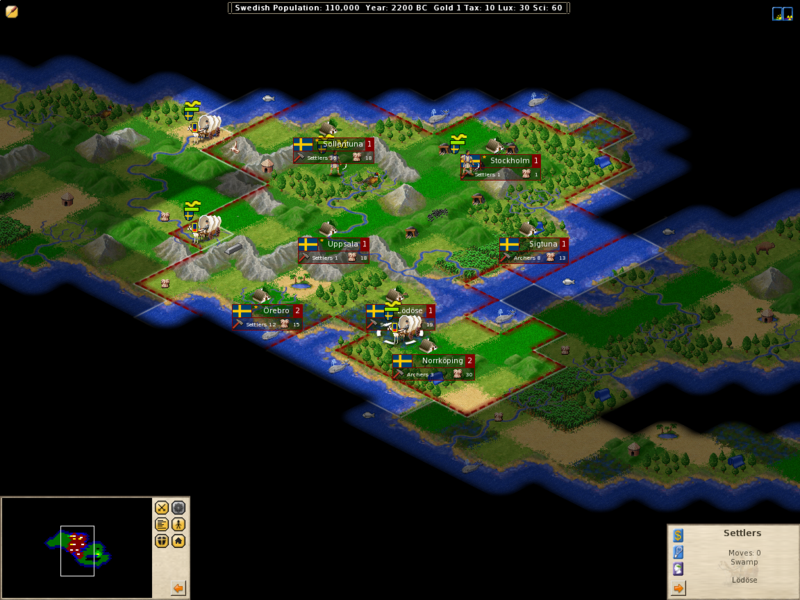
\includegraphics{Figures/Chapter1/minimap.png}
\decoRule
\caption[Overview Plus Details In Computer Games]{The computer game \emph{Freeciv} has a mini-map in the bottom left corner. This is a similar concept as \gls{opd}. On this mini-map the white rectangle represents the area of the map currently visible on the main screen. The different colors represent land and ocean and the territories of the different players. The white dots are the position of cities and the blackness are the unexplored areas (the ``fog of war'')\cite{wiki:minimap}.}
\label{fig:minimap}
\end{figure}

Note that the term of \emph{Overview + Details} sometimes are also referred to as \emph{Focus + Context}, \emph{Mini-map} or some other terms, however, they are referring to a similar techniques or concepts. 

%----------------------------------------------------------------------------------------
%	SECTION
%----------------------------------------------------------------------------------------

\section{Motivation For More Complicated Situations}

Most of these techniques and examples above are feasible and can improve how human comprehend the information or datasets is because the whole context area, although larger than how much one screen can hold, comparing to the focus area, is still not so much bigger. If you're looking at a street plan of a city, the focus area can still be visibly represented as a rectangle if the context area is only as large as a city. If you're looking at an image with the resolution of twice as wide and tall as your screen monitor, the focus area still has a quarter of the size of the context area.

However, there are situations when these techniques will not be able to improve our comprehension of the whole dataset in a very good way, that is when the resolution of the original dataset is getting too high and the focus area is zoomed in into an extremely detailed state. That way, the focus region becomes a ``dot'' instead of a region to be represented on the context view, losing its width and height properties and stops giving intuitive information. A simple example is shown in \gmref{fig:becomespoint} indicating that when the resolution of the dataset is extreme, new approaches need to be taken in order to let the users able to ``grab the whole picture''.

\begin{figure}[H]
\centering
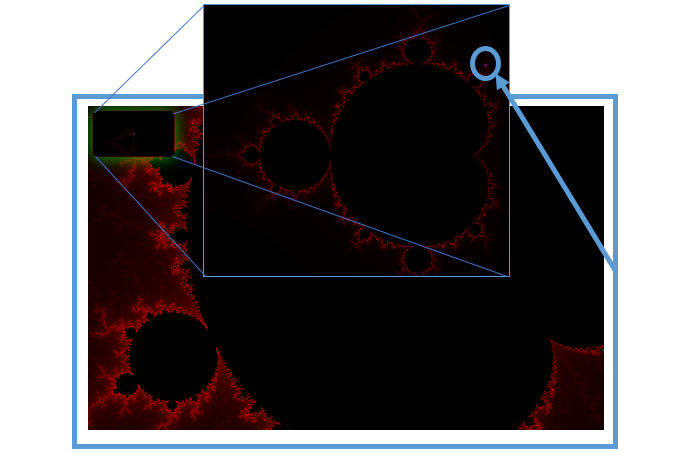
\includegraphics[width=0.9\textwidth,keepaspectratio]{Figures/Chapter1/becomespoint.png}
% 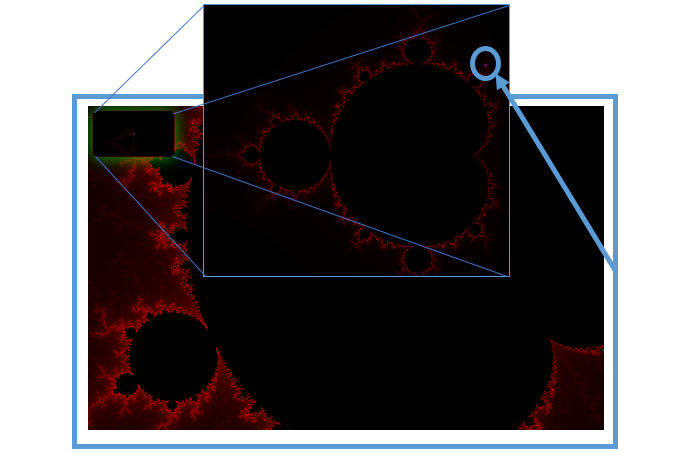
\includegraphics{Figures/Chapter1/becomespoint.png}
\decoRule
\caption[Focus Region Becomes A Dot On Context Region]{Traditional \gls{opd} techniques stop to provide intuitive information on a highly zoomed-in fractal image.}
\label{fig:becomespoint}
\end{figure}

In these situations, a new level of the \gls{opd} techniques is introduced, which is to provide more levels of overviews to the user. Take what's shown in \gmref{fig:zeus} as an example, multiple levels of information of objects are presented as overviews for the users to browse and search. For a similar solution as shown previously in \gmref{fig:becomespoint}, a solution shown in \gmref{fig:multiplelevels} is to give multiple hierarchical overviews to the user to preserve the intuitiveness of the techniques.

\begin{figure}[H]
\centering
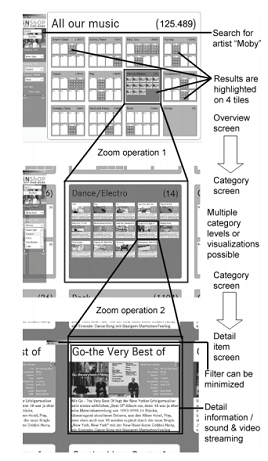
\includegraphics[width=0.35\textwidth,keepaspectratio]{Figures/Chapter1/zeus.png}
% 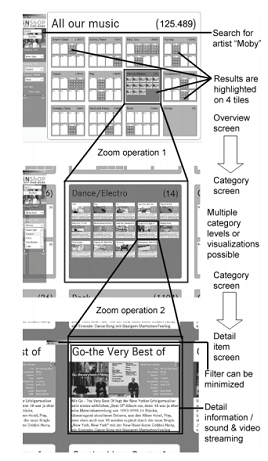
\includegraphics{Figures/Chapter1/zeus.png}
\decoRule
\caption[Multiple Levels of Overview Plus Details]{ZEUS from overview to detail view by zoom in\cite{gundelsweiler2007zeus}.}
\label{fig:zeus}
\end{figure}

\begin{figure}[H]
\centering
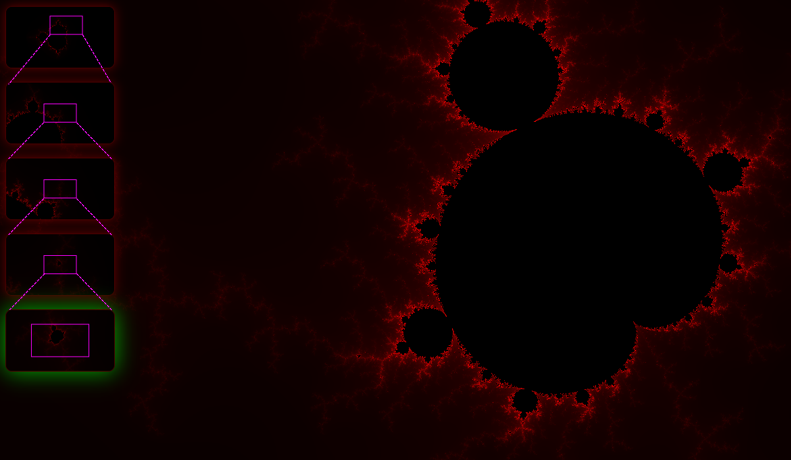
\includegraphics[width=0.9\textwidth,keepaspectratio]{Figures/Chapter1/multiplelevels.png}
% 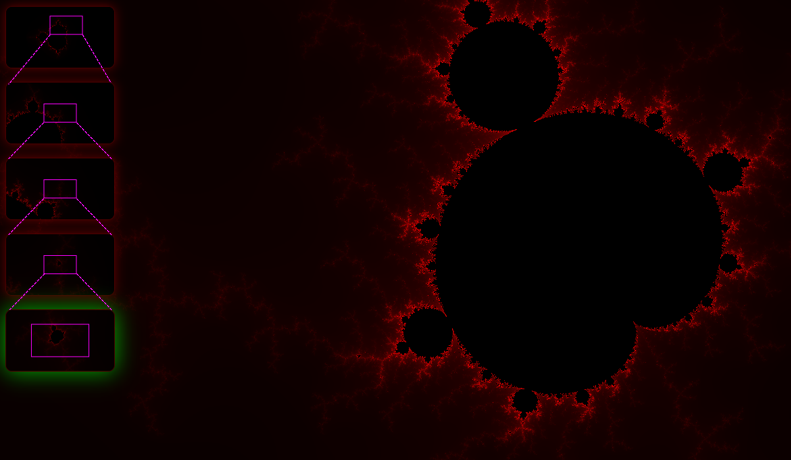
\includegraphics{Figures/Chapter1/multiplelevels.png}
\decoRule
\caption[Zoomed-in Fractal Image]{A graphical representation of Mandelbrot set zoomed in for around $35$ thousand times compared to the original.}
\label{fig:multiplelevels}
\end{figure}

This solution is straightforward, however, we can still raise questions to push the topic into new levels --- what happens when the resolution of the dataset increases even more?

In this case, more overviews need to be added and presented to the users. When more overviews are added providing more \glspl{lod} and contexts and put to the screen, the original problem emerges again --- these overviews are going to occupy a large portion even the entire screen monitor so the most zoomed-in detail area, the most important area of interest, is not going to be easily comprehended or even not able to be seen, as shown in \gmref{fig:occupiesscreen}. 

\begin{figure}[H]
\centering
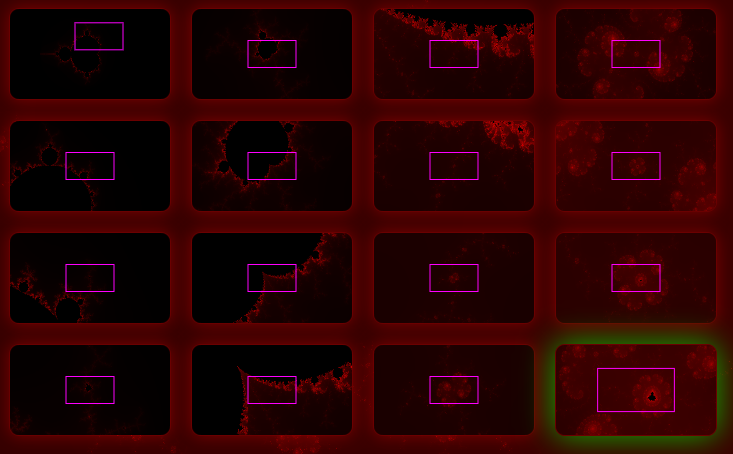
\includegraphics[width=\textwidth,keepaspectratio]{Figures/Chapter1/occupiesscreen.png}
% 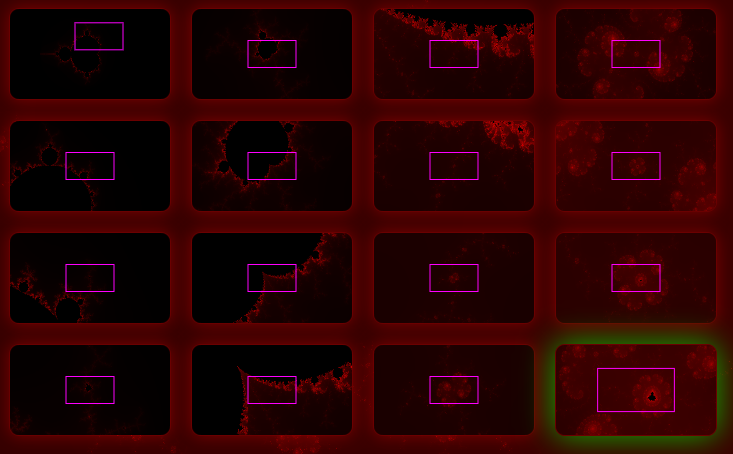
\includegraphics{Figures/Chapter1/occupiesscreen.png}
\decoRule
\caption[Occupied Screen]{Too many overviews occupying entire screen monitor.}
\label{fig:occupiesscreen}
\end{figure}

Therefore, the topic of this thesis is focused on solving this problem, to arrange these overviews in certain ways that they can all provide hierarchies of overviews of information with respect to the original extreme resolution dataset, at the same time, being intuitive enough for human users to understand the \glspl{lod} as well as the most detailed region with the help of all these arrangements.

\section{Inspirations for the Arrangements of Context Views}

\glsunset{it}

As we mentioned above, in order to prevent situations like shown in \gmref{fig:occupiesscreen} that all tiled context views occupying the entire focus view from happening, we figured out several ways of arranging these context views, and the inspirations of which came from various ways of how we interact with \gls{it} related objects.

\subsection{Dock And Scrollbar}

First thing that came into my mind was the state-of-the-art designs from \emph{Apple}. They invented the concept of macOS Dock or \emph{Dock} as shown in \gmref{fig:macosdock1}, which can be used as an idea of arranging multiple objects of interest on one screen. Not that as shown in \gmref{fig:macosdock1-1}, that it adds an eye-catching visual effect to the current focused object and some other coherent objects.

\begin{figure}[th]
\centering

\includegraphics[width=\textwidth,keepaspectratio]{Figures/Chapter1/macosdock1.png}
% 
\includegraphics{Figures/Chapter1/macosdock1.png}
\decoRule
\caption[MacOS Dock]{Apple gives users the ability to put interested Apps on one side of the screen, which can be the interested contexts in our project.}
\label{fig:macosdock1}
\end{figure}

\begin{figure}[th]
\centering
% 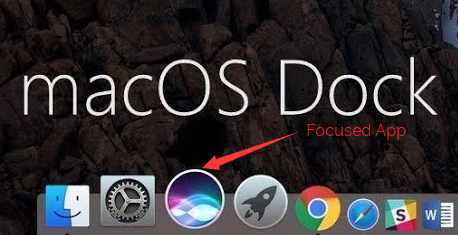
\includegraphics[width=\textwidth,keepaspectratio]{Figures/Chapter1/macosdock1-1.png}
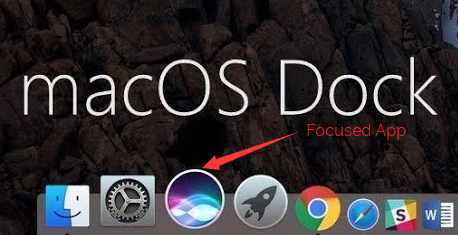
\includegraphics{Figures/Chapter1/macosdock1-1.png}
\decoRule
\caption[MacOS Dock Hover]{When user hovers over an object of interest on the Dock, the Dock can show a visually distinguishable effect.}
\label{fig:macosdock1-1}
\end{figure}

However, in situations that when user tries to add more interested objects to the Dock, this design only shrinks the sizes of the objects and cannot provide capabilities to embody more objects and advance further, as shown in \gmref{fig:macosdock2}.

\begin{figure}[th]
\centering

\includegraphics[width=\textwidth,keepaspectratio]{Figures/Chapter1/macosdock2.png}
% 
\includegraphics{Figures/Chapter1/macosdock2.png}
\decoRule
\caption[MacOS Dock With More Apps]{Apple Dock has certain limitations of holding more objects inside.}
\label{fig:macosdock2}
\end{figure}

At the same time, to display more object in a smaller container, there is an obvious way of putting a scrollbar beside it, as shown in \gmref{fig:scrollbar}. Therefore, the first idea of combining a scrollbar together with the visual effects of the macOS Dock were formed.

\begin{figure}[H]
\centering
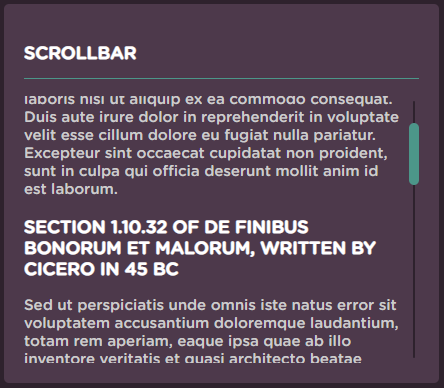
\includegraphics[width=.5\textwidth,keepaspectratio]{Figures/Chapter1/scrollbar.png}
% 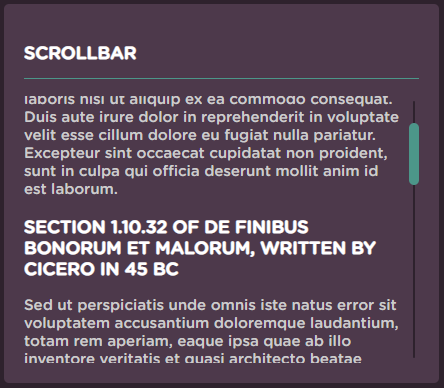
\includegraphics{Figures/Chapter1/scrollbar.png}
\decoRule
\caption[Modern-looking Scrollbar]{An example of using a scrollbar on the side of a container to allow users to browse through more information inside this container.}
\label{fig:scrollbar}
\end{figure}

\subsection{Stacked Cards}

We all browse through different web pages for some information nowadays, and we all had the necessity to keep several web pages open at the same time at some point. The amount of opened websites can easily grow out of hand and how the modern web browsers are handling these web pages of interest can easily catch our attention. The next thing that caught my attention is the \emph{iOS Safari} browser. It is a famous browser installed by default on a popular mobile phone which is a device that has limited amount of space for visual area. How it's displaying the opened web pages are shown in \gmref{fig:iossafari}.

Visually, they look like cards stacked upon each other. What if we arrange it in a way that this stack of cards can dynamically adjust their positions on screen and the angles they pile up with as their numbers grow? This can be the next good way of arranging these context views of our project.

\begin{figure}[th]
\centering
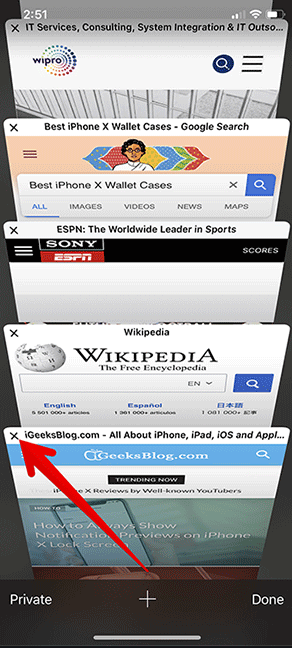
\includegraphics[width=.4\textwidth,keepaspectratio]{Figures/Chapter1/iossafari.png}
% 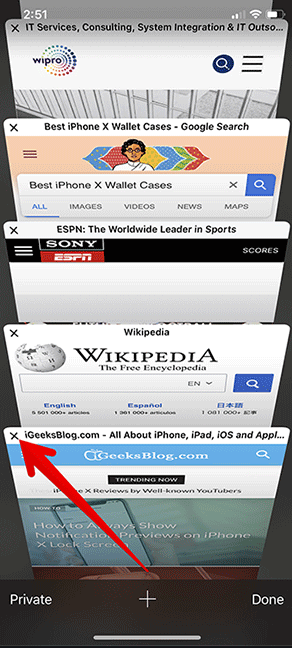
\includegraphics{Figures/Chapter1/iossafari.png}
\decoRule
\caption[Means of Arrangements On iOS Safari]{How iOS Safari arranges multiple open web pages on an iPhone.}
\label{fig:iossafari}
\end{figure}

\subsection{Tabs}

As mentioned before, how browsers arrange the open web pages can be really good examples for our project, therefore, we can't neglect the conventional way of arranging the open web pages on the top of the visual area as ``opened tabs'', like shown in \gmref{fig:tabs}. This is the third idea of cases we make in this project.

\begin{figure}[H]
\centering

\includegraphics[width=\textwidth,keepaspectratio]{Figures/Chapter1/tabs.png}
% 
\includegraphics{Figures/Chapter1/tabs.png}
\decoRule
\caption[How Google Chrome Arranged Objects of Interest]{The way Google Chrome handles the open web pages are to put a so-called ``tab'' on top of visual area shaped like a tag, with informative titles which sometimes are shortened with ellipsis at the end.}
\label{fig:tabs}
\end{figure}

\subsection{Previews Of Contexts}

\glsunset{pc}

As shown in \gmref{fig:multiplelevels}, the context views can be relatively small when put to action. Therefore, we need some sort of mechanism to let the user ``preview'' the shrunk context views, in a similar sense where \emph{Windows 10} users can hover their cursor over the bottom right corner of their screen monitor to have a ``glance'' of how their desktop looks like shown in \gmref{fig:winpreview}, hiding the \gls{ui} of the current open applications.

\begin{figure}[H]
\centering
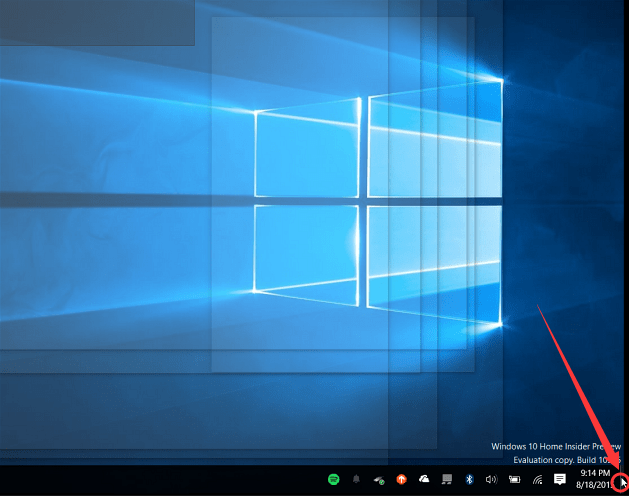
\includegraphics[width=\textwidth,keepaspectratio]{Figures/Chapter1/winpreview.png}
% 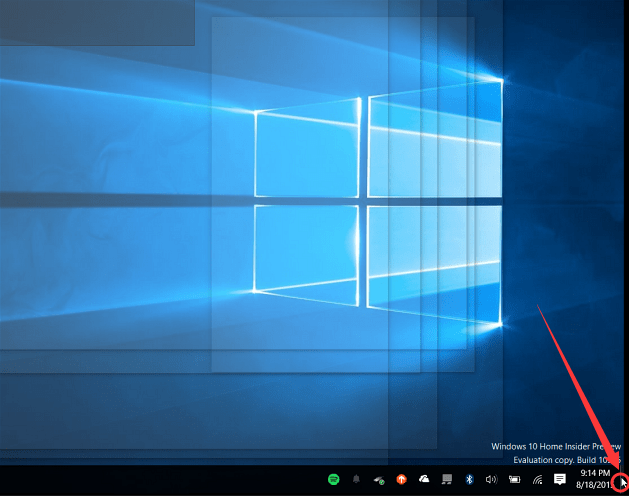
\includegraphics{Figures/Chapter1/winpreview.png}
\decoRule
\caption[``Preview'' Mechanism on Windows 10]{When users hover their mouse cursor on bottom right corner of a Windows \gls{pc} and have a glance of what is on their Desktop.}
\label{fig:winpreview}
\end{figure}

A most natural preview setup would be like this, when the user hovers over one of the context view, display an enlarged image in \gls{fhd} that shows the context. That is in fact the default setting of this project.

As inspired by the same \emph{Windows} effect, the second visual effects type becomes a fade-in and fade-out effect. This effect, as shown in \gmref{fig:jqfadein}, is adding a small transition in the transparencies of the context to be displayed on screen --- smoother and can give positive user experience in the comprehension of the \gls{fpc} problem.

\begin{figure}[H]
\centering
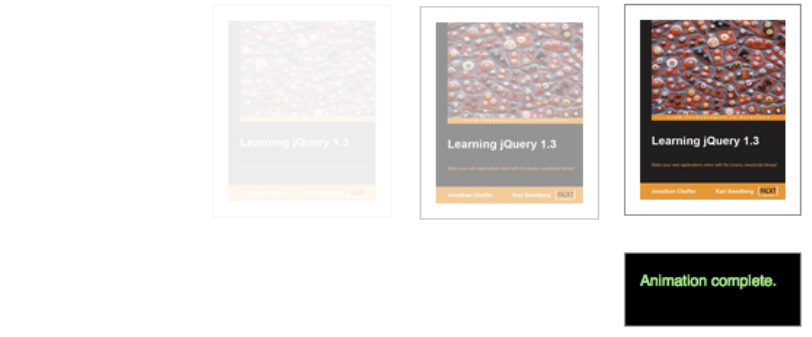
\includegraphics[width=\textwidth,keepaspectratio]{Figures/Chapter1/jqfadein.png}
% 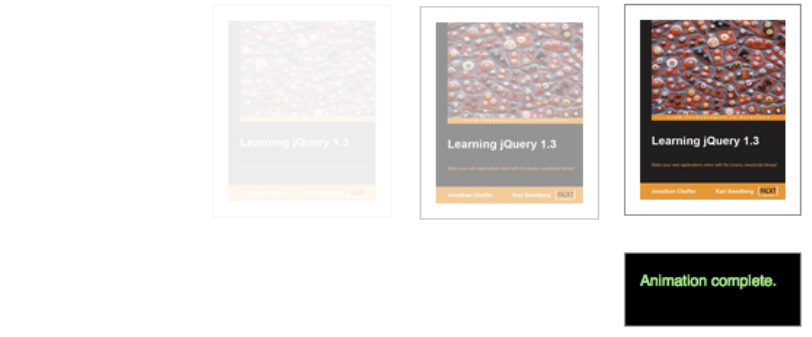
\includegraphics{Figures/Chapter1/jqfadein.png}
\decoRule
\caption[Fade-in Effect in jQuery]{Illustration of the \texttt{fadeIn()} effect in \emph{jQuery}, a transparency change of objects to be displayed.}
\label{fig:jqfadein}
\end{figure}

Another way of giving previews of the contexts is inpired by some modern graphics and video work, such as a deep zooming video of Mandelbrot set\footnote{ See \url{https://www.youtube.com/watch?v=pCpLWbHVNhk} for more information.} or some special scenes in a movie such as Limitless\footnote{ See \url{https://www.youtube.com/watch?v=xqv1maJaDtQ&t=37} for more information} or Man In Black\footnote{ See \url{https://www.youtube.com/watch?v=OKnpPCQyUec} for more information.}.

As shown in \gmref{fig:zoompreview}, it would be really nice if we implement this visual feature that when user wants to preview one of the contexts, instead of magically showing that context, we show this process of letting the preview image raise or sink from the ``current'' depths to the ``intented'' depths of the context. Therefore, this second ways of previewing the contexts got to be implemented into this project.

\begin{figure}[H]
\centering
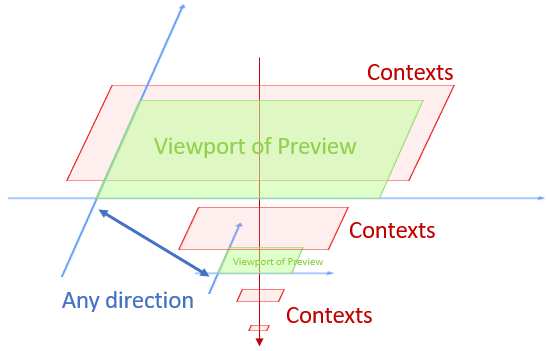
\includegraphics[width=.8\textwidth,keepaspectratio]{Figures/Chapter1/zoompreview.png}
% 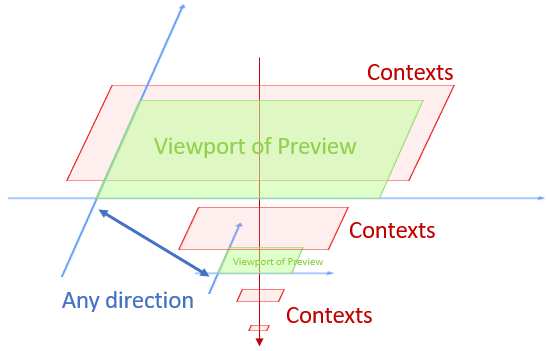
\includegraphics{Figures/Chapter1/zoompreview.png}
\decoRule
\caption[Moving Preview Plane On Context Views]{The viewport of preview is like a plane raising or sinking to the desired depths on the \texttt{z} axis.}
\label{fig:zoompreview}
\end{figure}

%----------------------------------------------------------------------------------------
%	SECTION
%----------------------------------------------------------------------------------------

\section{Related Work}

There are many researchers who have already done plenty of work related to the topic of \gls{opd}, \gls{fpc} or \gls{lod}.

Some researchers did work on a single level of \gls{fpc} techniques:

Cockburn et al. \cite{cockburn2006review}\cite{cockburn2009review} reviewed and compared \gls{opd}, zooming, and \gls{fpc} interfaces. They described that \gls{opd} uses a spatial separation between focused and contextual views, zooming is temporal separation of views and \gls{fpc} displays the focus within the context.

Hornb{\ae}k et al. \cite{hornbaek2002navigation} compared zoomable user interfaces with and without an overview by experiments to understand the navigation patterns and usability of these interfaces. In a later work, Hornb{\ae}k et al. \cite{hornbaek2011notion} extensively reviewed papers that used the notion of overview and developed a model which highlights the awareness that makes up an overview, the process, by which users acquire it, the usefulness of overviews, and the role of user-interface components in developing an overview.

In \cite{baudisch2002keeping} considered Baudisch et al. mainly the technique focus plus context screens. They experimented and compared this technique with the other two techniques overview plus detail and zooming/panning. They noted, for interaction with dynamic views, the technique focus plus context screens alone seems not to be enough and needs an additional monitor. In a related work, Baudisch et al. \cite{baudisch2001focus} present the technique focus plus context screens and implemented a system with this technique by combining multiple display units of different resolution. Their means is particularly suitable for situations where all information is shown in only one view and switching between multiple views should be avoided.

Roto et al. \cite{roto2006minimap} developed a Web page visualization method minimap for mobile phones that shows pages in a modified original layout and navigates a Web page with a mini map view.

Gutwin et al. \cite{gutwin2004interacting} compared three techniques: fisheye, zoom and panning, to find out what is the best ways to redesign a large UI to fit a smaller screen of mobile devices.

Holmquist \cite{holmquist1998zoom} developed a flip zooming as a new focus+context technique: Mini Pages are placed in a simple left-to-right, top-to-bottom ordering on the display. When a page is brought into focus, it is enlarged and placed approximately in the middle of the display, with the other Mini Pages arranged around it.

There are also some researchers did work related with multiple \glspl{lod}:

Pan et al. \cite{zhigeng1998overview} present a summary on the mesh simplification techniques which they used for creating models at multiple \gls{lod}. In this paper they also compared typical methods.

Clark \cite{clark1976hierarchical} proposed hierarchical geometric models for visible surface algorithms for producing computer pictures. He described the benefits of using more than one representation of a model for image rendering and pointed out that objects that cover a small area of the screen can be rendered from a simplified version of the object and that this allows more efficient rendering of a scene.

Crow described the benefits of having both simple and complex representations of an object in his paper on an image generation environment.\cite{crow1982more} He gave an example of a chair that is represented in high detail, medium detail and very low detail. These models with three level of detail were created by hand. He suggested that creating the lower levels of detail is a process that should be automated.

Gundelsweiler et al. \cite{gundelsweiler2007zeus} developed a system of hierarchical information structure. Objects and categories are organized in groups on different hierarchy level visualized as tiles on the screen by the user. The search is supported by zooming/panning navigation.


% ---

% Single level:

% 1. A Review of Overview+Detail, Zooming, and Focus+Context Interfaces\cite{cockburn2009review}

% 2. A Review of Focus and Context Interfaces\cite{cockburn2006review}

% 3. Navigation Patterns and Usability of Zoomable User Interfaces with and without an Overview\cite{hornbaek2002navigation}

% 4. Keeping Things in Context: A Comparative Evaluation of Focus Plus Context Screens, Overviews, and Zooming\cite{baudisch2002keeping}

% 5. Focus Plus Context Screens: Combining Display Technology with Visualization Techniques\cite{baudisch2001focus}

% 6. Minimap – A Web Page Visualization Method for Mobile Phones\cite{roto2006minimap}

% 7. Interacting with Big Interfaces on Small Screens: a Comparison of Fisheye, Zoom, and Panning Techniques\cite{gutwin2004interacting}

% 8. The notion of overview in information visualization\cite{hornbaek2011notion}

% 9. The Zoom Browser: Showing Simultaneous Detail and Overview in Large Documents\cite{holmquist1998zoom}


% Multiple level:

% 10. Overview of Multiple Level of Detail Creation\cite{zhigeng1998overview}

% 11. Hierarchical geometric models for visible surface algorithms\cite{clark1976hierarchical}

% 12. A more flexible image generation environment\cite{crow1982more}

% 13. ZEUS–zoomable explorative user interface for searching and object presentation\cite{gundelsweiler2007zeus}